\documentclass[a4paper, 11pt]{article}
\usepackage[top = 1.2in, bottom = 1.2in, left = 0.6in, right = 0.6in]{geometry}
\usepackage{amsmath}
\usepackage{graphics}
\usepackage{graphicx}
\usepackage{subcaption}
\usepackage{caption}
\usepackage{listings}
\usepackage{multirow}
\usepackage{url}
\usepackage[labelfont=bf]{caption}

\begin{document}

%%Title
\Large
\begin{center}
\hrulefill \\
\textbf{IMAGE PROCESSING} \\
SF2 - FIRST INTERIM REPORT \\
\vspace{0.2cm}
\normalsize 
Quang-Thinh Ha - CRSid: qth20 \\
\hrulefill \\
\end{center}

\normalsize

\section{Introduction}

This project aims at developing an algorithm for image compression, while preserving the quality of the decompressed image at an acceptable level. \\
\noindent
The first week aims at delivering basic foundation techniques, including \textit{image filtering}, building \textit{Laplacian Pyramid} and \textit{quantisation} for \textit{efficient coding}. The observations on these particular areas are mentioned on this first interim report. 

\section{Simple Image Filtering}
An effective image low-pass filter, of \textit{odd} length $\mathit{N}$, ma be ontained by defining the impulse response $\mathit{h(n)}$ to be a sampled half-cosine pulse:

\begin{equation*}
\mathit{h(n) = G cos \big( \frac{n \pi}{N+1} \big)} \, \, \, \mathrm{for} \mathit{\frac{-(N-1)}{2} \leq n \leq \frac{N-1}{2}}
\end{equation*}
\noindent
and for unity gain at zero frequency, the gain factor \textit{G} should be calculated that: $ \sum\limits_{n=-(N-1)/2)}^{(N-1)/2} h(n) = 1 $ \\
\noindent
It is deduced that the larger the value of \textit{N}, the wider the half-cosine pulse would be. The larger the half-cosine pulse is, the 'lower-pass' the filter is, which results in blurrier images.This is demonstrated by Figure 1 in the Appendix. \\
\noindent
The blurrier the image, the number of components in low-pass filtered images decreases, leading to decrease in energy for low-pass filtered image. As theses components are filtered into high-pass filtered image, they contribute to the rise in energy here instead.
\noindent
As an images with finite size, the edges of the image is represented with high frequency components (just like a 'sharp' step signal). In order to minimise the edge effects, a technique called \textit{symmetric extension} is applied, in which it is assumed that there are flat mirror along each edge of the image. The filtered image will also be symmetrically extended in all directions with the same period as the original images. \\
\noindent
Due to this property of symmetry, there should not be any differences whether the rows or columns are filtered first. However, the maximum absolute pixel difference between row-column and column-row filtered images, obtained from MATLAB, is $\mathbf{1.1369\times10^{-13}}$. This is insignificant, and the presence of this tiny numerical error can be explained due to the discretisation of the convolving process in MATLAB. 
\section{Laplacian Pyramid}
The goal of image pyramid is to develop filter-based representations to decompose images into information at multiple scales, which are natural for image coding (Figure 2). This concept will be explained further in the following section. Reconstruction of the original image can then be down by using the smallest low-pass filtered image, combined with the smallest high-pass filtered image and `climb up' in the pyramid again. Images at further depth down the pyramid, if scaled to the same size as the original image, will be blurrier. The deepest one (which is way too small to visualise here) consist of 2x2-pixel image, with different shades of gray on each pixel. \\
\noindent
Other application for Laplacian pyramid includes image stitching and enhancement. Interesting features extracted at each level of the pyramid might be combined together into one final image. This area might be explored later on. 

\section{Quantisation and Coding Efficiency}
In order to figure out the approximate number of bits required to code the image pyramid, the entropy of the quantised image data needs to be calculated, as this represents the minimum average number of bits per sample needed to code samples. \\
\noindent
Quantised images will have lower entropy that non-quantised ones. This can be explained simply by thinking that 'smooth' data (those without quantisation) consists of several small tiny quantise steps. More steps means more information, and more information leads to higher entropy. Additionally, compared to low-pass filtered images, high-pass filtered images consists of fewer grey intensities, leading to less information is required to represent them. Hence, high-pass filtered images should have lower entropy, and this is confirmed in the lab. Data is not listed here for the sake of brevity. \\
\noindent
Before dwelling further on the topic of entropy, let's first discuss the effects of quantisation, and how quantisation at different number of layers on the pyramid affects the rms between the input and compressed image (Figure 3).  Output image of reconstruction that goes through more layers of quantised Laplacian pyramid contains larger RMS error. This is due to quantisation error will be magnified through the number of layers. \\
\noindent
Furthermore, a quantise step of, for example, 8 at image depth 4 on the pyramid, will not remain the same at image depth 3 - in fact the quantise step for the image at depth 3 should be larger. This statement also contributes for the increase in RMS error, and will be fixed using \textit{equal MSE scheme} instead. \\
\noindent
Examining the top row Figure 4 will allow us to clearly observe the changes in the artefacts of the output image when more layers of the pyramid are generated. The cloud is washed out more as the number of layers increases. This might not be a bad trade, as most of the fine details of the pictures (the lighthouse, the fences etc.) are still represented nicely. \\
\noindent
Paying closer attention to the two row of Figure 4 - which is generated using constant quantise step scheme - and the bottom row ones - generated using equal MSE scheme. Using the quantise step schemes, the difference between the fourth and fifth images is unnoticeable, considering only an improvement of compression ratio from $\mathbf{1.2485}$ to 1.2489 only. Hence, for this scheme, \textit{the optimise number of layers is 4.} Same deduction is made for the equal MSE scheme, with a compression ratio of $\mathbf{1.5494}$ instead. \\
\noindent
The same observation, that equal MSE scheme provides higher compress ratio compared to constant quantise step scheme, is also achieved when an alternative, more complicated filter is used instead\footnote{Based on the notation from the handout, $m = 4$.}. From the graph of Figure 5, an optimise choice for constant quantise step is using \textit{two layers} with a compress ratio of \textbf{1.33}. Using equal MSE scheme gives an optimal choice of \textit{three layers} for compression ratio of \textbf{1.4294}. Hence, using this alternative filter offers better compress ratio for the algorithm.\\
\noindent
There is one strange trend on the plot of compress ratio against number of layers in one specific case, in which the plot is coloured red in Figure 5. Instead of following similar trend like others - the ratio plateaus after a certain number of layers, the compression ratio drops after an initial rise, followed by a weak recovery in the end. Even though the optimise value for the number of layers still follow the previous argument nicely, this unexpected trend is quite interesting. The downward trend in compression ratio indicates that image is compressed `less' when more layers are used for constant step scheme coupled with the more complicated filter. This might mean using more layers might not always be a good choice for image compression algorithm. An educative guess would be due to the non-linearisation quantise step when using the same step size from one layer to another. Further investigation would be required here. 



\newpage
\section*{APPENDIX}
\begin{figure}[h]
\begin{center}
	\begin{subfigure}[b]{0.3\textwidth}
		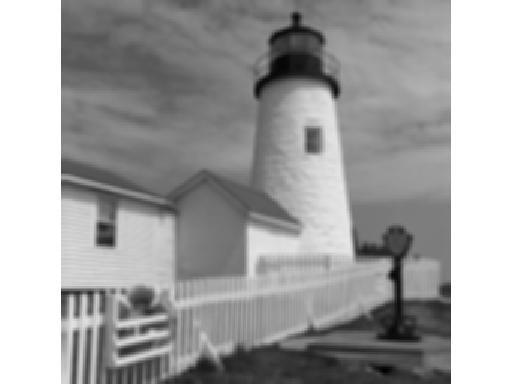
\includegraphics[width=\textwidth]{h_5.jpg}
		\caption{Length 5}
	\end{subfigure}
	\begin{subfigure}[b]{0.3\textwidth}
		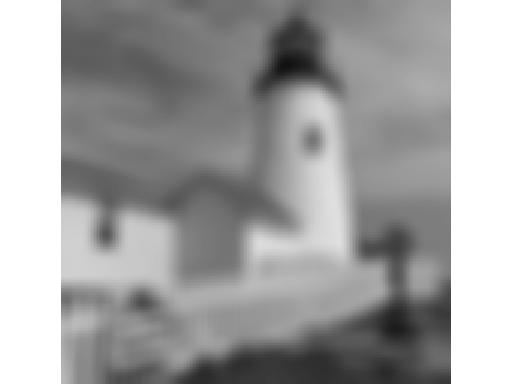
\includegraphics[width=\textwidth]{h_19.jpg}
		\caption{Length 19}
	\end{subfigure}
	\begin{subfigure}[b]{0.3\textwidth}
		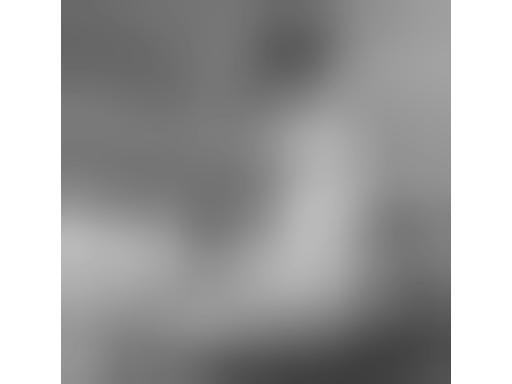
\includegraphics[width=\textwidth]{h_80.jpg}
		\caption{Length 80}
	\end{subfigure}
	\caption{\textbf{Effect of different odd-length half-cosine filters.} These images are filtered in both direction, so the original picture is `blurred symmetrically'. }
\end{center}
\end{figure}
\begin{center}
\begin{tabular}{|c | c | c|}
\hline
\textbf{\textit{N}} & \textbf{Low-Pass Filtered} & \textbf{High-Pass Filtered} \\
\hline
11 & 1.2631e09 & 4.0927e07 \\
\hline
13 & 1.2593e09 & 4.4806e07 \\
\hline
15 & 1.2560e09 & 4.7950e07 \\
\hline
17 & 1.2529e09 & 5.0450e07 \\
\hline 
19 & 1.2501e09 & 5.2509e07 \\
\hline
\end{tabular}
\captionof{table}{\textbf{Observation on energy of low-pass and high-pass filtered images' energy at different length of half-cosine pulse}. Common images, the high-frequency energy is much less than the low-frequency energy, and this is illustrated clearly in these figures. Another interesting feature is as N increase, low-pass filtered energy drops along with rises in high-pass filtered energy. }
\end{center}

\begin{center}
\begin{figure}[h]
\begin{center}
	\begin{subfigure}[b]{0.4\textwidth}
		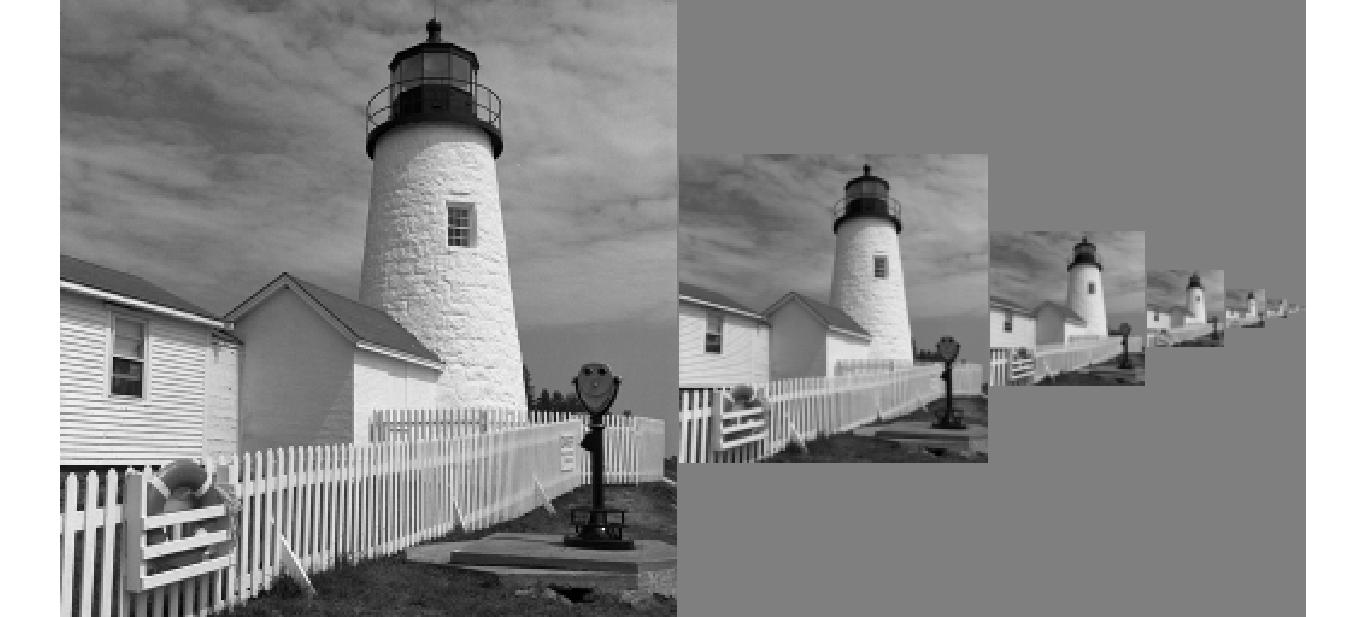
\includegraphics[width=\textwidth]{x_cell_pyramid.jpg}
		\caption{Low-pass images.}
	\end{subfigure}
	\begin{subfigure}[b]{0.4\textwidth}
		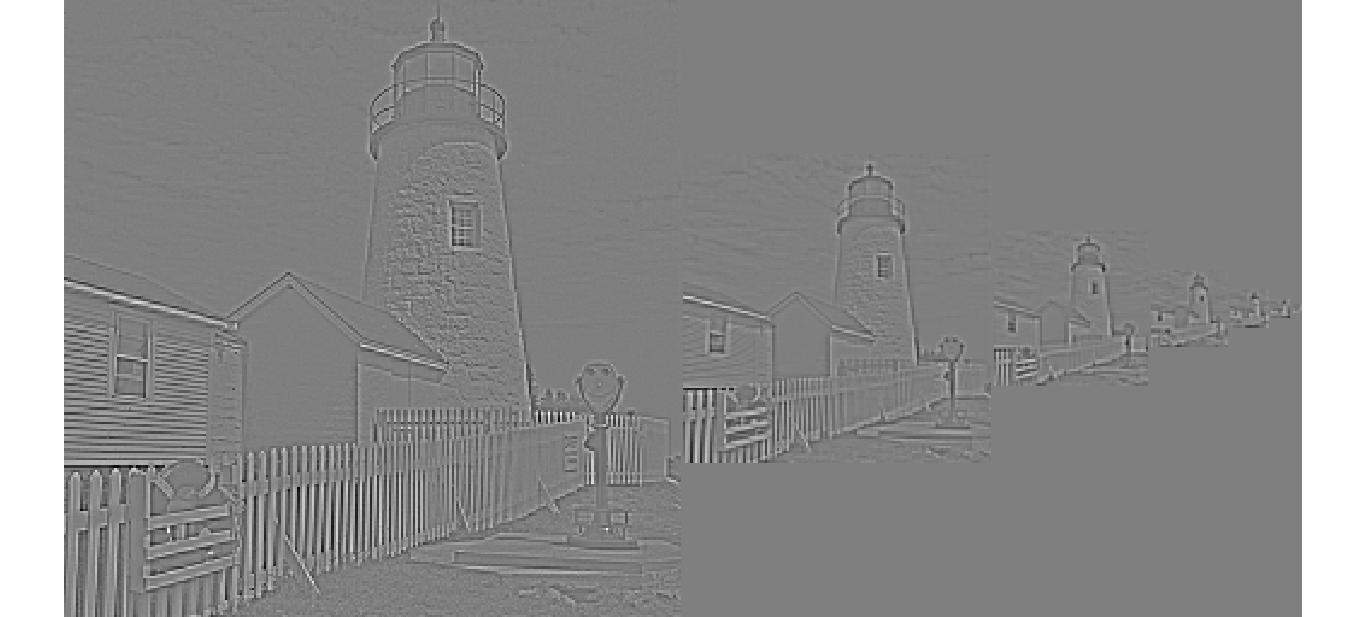
\includegraphics[width=\textwidth]{y_cell_pyramid.jpg}
		\caption{High-pass images. }
	\end{subfigure}
	\caption{\textbf{Laplacian pyramids consist of high-pass and low-pass images.} Both are at the furthest possible depth down (7). Images at further depth down the pyramid, if scaled to the same size as the original image, will be blurrier. The deepest image (which is way too small to visualise here) consist of 2x2-pixel image, with different shades of gray on each pixel. }
	\end{center}
\end{figure}
\end{center}

\begin{center}
\begin{figure}[h]
\begin{center}
	\begin{subfigure}[b]{0.3\textwidth}
		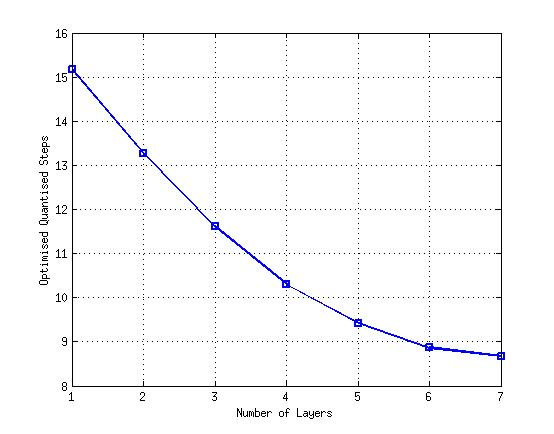
\includegraphics[width=\textwidth]{optimised_quantise_against_layers.jpg}
		\caption{Optimised Quantise Steps}
	\end{subfigure}
	\begin{subfigure}[b]{0.3\textwidth}
		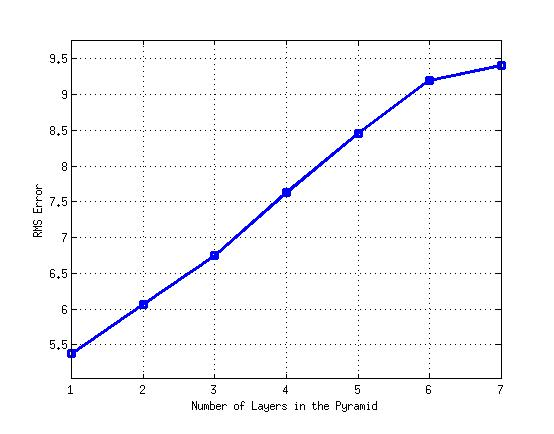
\includegraphics[width=\textwidth]{rms_against_layers.jpg}
		\caption{RMS Error}
	\end{subfigure}	
	\end{center}
	\caption{\textbf{Effect on quantisation over more layers on image reconstruction.} Using more layers to reconstruct the output image from quantised Laplacian pyramid results in greater RMS error. The optimised quantised step to obtain the same RMS error as the quantised original image decreases when reconstruction goes through more layers, and seems to plateau at a value.}
\end{figure}
%\begin{figure}[h]
%\begin{center}
%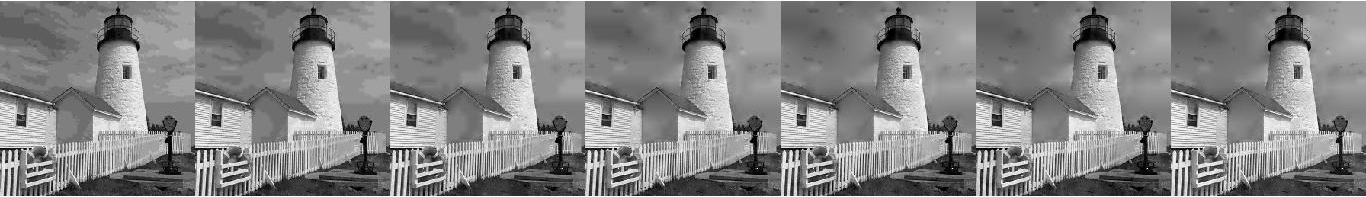
\includegraphics[width=\textwidth]{pyramid_output.jpg}
%\caption{\textbf{Visual artefacts on output images against the depth of the Laplacian pyramid for reconstruction}. The artefacts between 6-layer and 7-layer pyramids are relatively indifferent. This may explains why, on the graph of Figure 3(b), the gradient for the increase in RMS error from 6- to 7-layer pyramid suddenly decreases. }
%\end{center}
%\end{figure}
\begin{figure}[h]
\begin{center}
	\begin{subfigure}[b]{0.8\textwidth}
		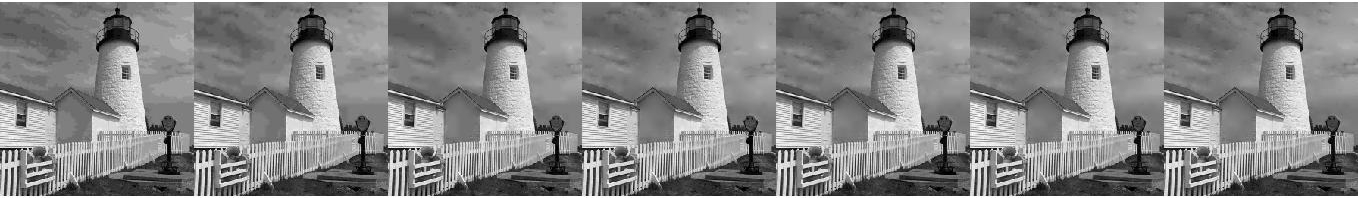
\includegraphics[width=\textwidth]{image_const_q.jpg}
	\end{subfigure}
	\begin{subfigure}[b]{0.8\textwidth}
		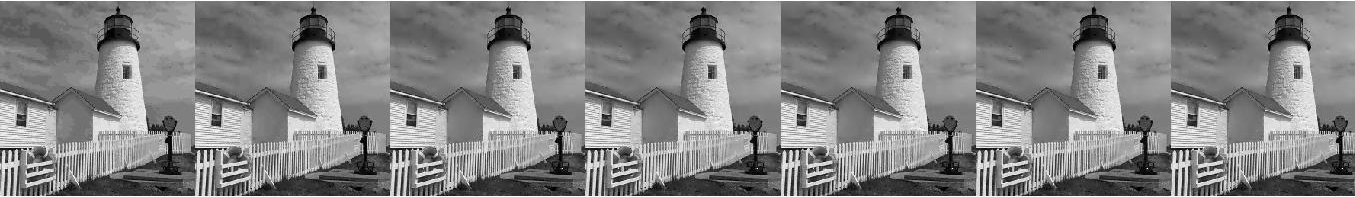
\includegraphics[width=\textwidth]{image_adjust_q.jpg}
	\end{subfigure}
	\caption{\textbf{Visual quality on reconstructed images using different schemes.} In the constant quantise steps (top), there is not much improvement in image quality after 4 layers, so this is chosen as the optimise number of layers. For \textit{equal MSE scheme}, the best compression ratio, with relatively good image quality, is presented after 4 layers. These images are generated using filter of $m = 2$.}
\end{center}

\end{figure}

\begin{figure}[h]
\begin{center}
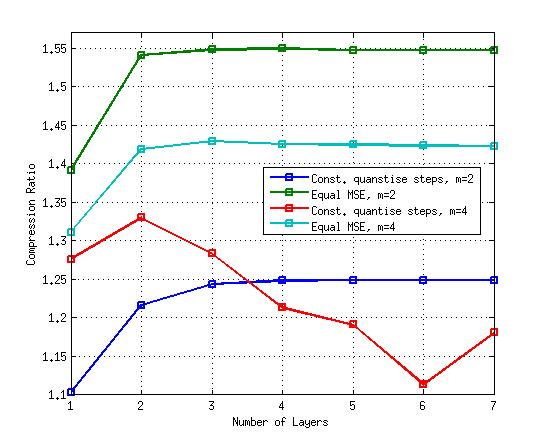
\includegraphics[width=0.45\textwidth]{compress_ratio.jpg}
\caption{\textbf{Variation on compression ratio over number of layers, using different schemes.} There seems to be some interesting changes for the compression ratio against number of layers in the constant quantise step scheme using the filter with $m = 4$.}
\end{center}
\end{figure}
\end{center}
\end{document}
